% !TEX encoding = UTF-8 Unicode
\chapter{Konzepte}
Die Konzepte welche Esper verwendet werdet, dienen dazu, den kompletten Ereignisfluss von der Aktion bis zur Verarbeitung und nachfolgenden Aktionen, abzubilden.
Ereignisse werden dezentral gefeuert und sind, durch die Registrierung der Ereignistypen auf dem Ereignis-Prozessor, klar definiert. Je nach hinterlegtem Regelwerk, werden diese, von einer Event-Engine, erfasst und verarbeitet oder ignoriert. Zur Regeldefinition dienen Muster, welche als Statements umgesetzt werden. Die Ereignismuster können verschiedene Techniken verwenden, nach denen der Ereignisstrom untersucht wird. 
Wie die Konfiguration, mit Ereignisdefinition-, Registrierung, sowie das Feuern und Verarbeiten der Ereignisse, in Esper umgesetzt wird, ist in Kapitel \ref{kapitel_architektur} beschrieben.
Nähere Informationen zu den Konzepten und weitere, hier nicht näher erläuterte, Möglichkeiten von Esper können der Dokumentation \cite{EsperRef2018} entnommen werden.
Im folgenden werden die Konzepte von Esper erläutert. Anschließend wird jeweils Bezug auf einen Casino-Anwendungsfall genommen und aufgezeigt.


\section{Statements}
\label{statements}
Statements dienen dazu Muster zu definieren, mit deren Hilfe die Event-Engine den Datenstrom analysiert. Hierzu existiert die \acf{EPL}, welche stark an den Syntax von SQL erinnert. Mit ihr werden die Ereignismuster definiert und die Ereignisverarbeitung umgesetzt.
\cite{EsperRef2018}[7-8]

\section{Select}

Quelltext \ref{basic_select} zeigt ein einfaches Select-Statement. Resultierend hieraus, wird der \acf{EP} auf alle Ereignisse vom Typ \texttt{Action} reagieren und diese bei Eintritt erfassen. 
\begin{lstlisting}[caption={Statement einfache Selektion}\label{basic_select},captionpos=b,language=SQL]

select * from GameActionEvent

\end{lstlisting}
Der Ablauf wird beispielhaft in Abbildung \ref{basic_select_img} grafisch dargestellt. Sie werden unverändert weitergegeben. Dieses Statement wird im dem Casino eingesetzt, um über sämtliche Züge informiert zu werden. Erkennbar ist jedoch nicht, welcher Zug zu welchem Spiel, etc. gehört. Um Ereignisse feingranular untersuchen zu können, werden weitere Techniken benötigt, welche beispielsweise nach Attributen filtern können.
\cite{EsperRef2018}[8-9]

\begin{figure}[h]
	\centering
	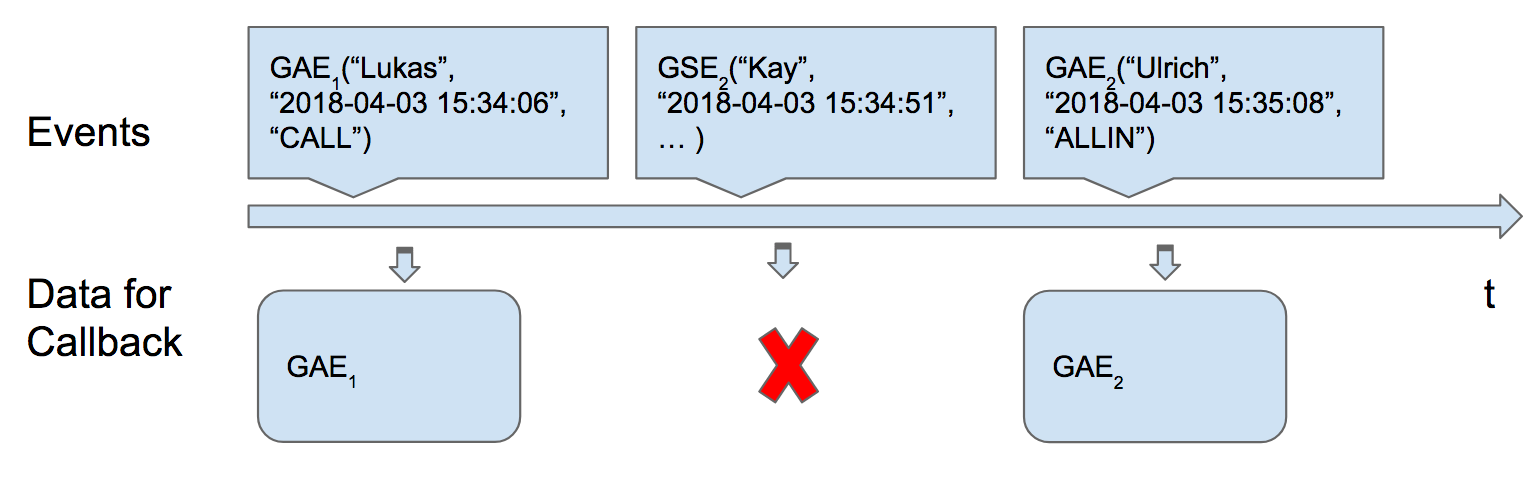
\includegraphics[width=\textwidth,height=\textheight, keepaspectratio]{images/statement_basic_select.png}
	\caption{Ablauf einfache Selektion}
	\label{basic_select_img}
\end{figure}

\section{Filter}

Die Filterfunktion ist eine geeignete Möglichkeit, die Selektion aus dem Ereignisfluss auf bestimmte Attribut-Werte zu beschränken. Wie das Beispiel in Quelltext \ref{filter_select} veranschaulicht, können, wie im SQL Syntax, Ereigniseigenschaften beschränkt werden.
\begin{lstlisting}[caption={Statement mit Filter}\label{filter_select},captionpos=b,language=SQL]

select playerName, deck from GameEndEvent(deck="ROYAL_FLUSH")

\end{lstlisting}
Wie Quellcode (\ref{filter_select}) zeigt, selektiert die Event-Engine die Attribute \texttt{playerName} und \texttt{deck} der auftretenden Ereignisse vom Typ \texttt{GameEndEvent}. Anschließend wird mit \texttt{GameEndEvent(deck="ROYAL\_FLUSH")} überprüft, ob der Wert des Deck-Attributes im Endevent, einem Royal-Flush entspricht.
Der Ablauf des Quellcodes wird in Abbildung \ref{filter_select_img} grafisch aufgezeigt. Gut zu sehen, ist, dass nur die End-Events erfasst werden, welche dem Attribut-Wert entsprechen. Weil nur ein Spieler mit einem Royal-Flush-Blatt gewinnt, wird auch nur dieses Ereignis verarbeitet.
Das Casino benötigt ein solches Statement, um zu erfahren, wer welches Spiel mit welcher Hand gewonnen wird. Um jedoch, einen Spieler mit oftmaligem Glück zu entdecken, ist die Anzahl der Siege erwünscht. Hierfür können die selektierten Daten, mit weiteren Funktionen aggregiert werden.
\cite{EsperRef2018}[10-11]
\begin{figure}[ht]
	\centering
	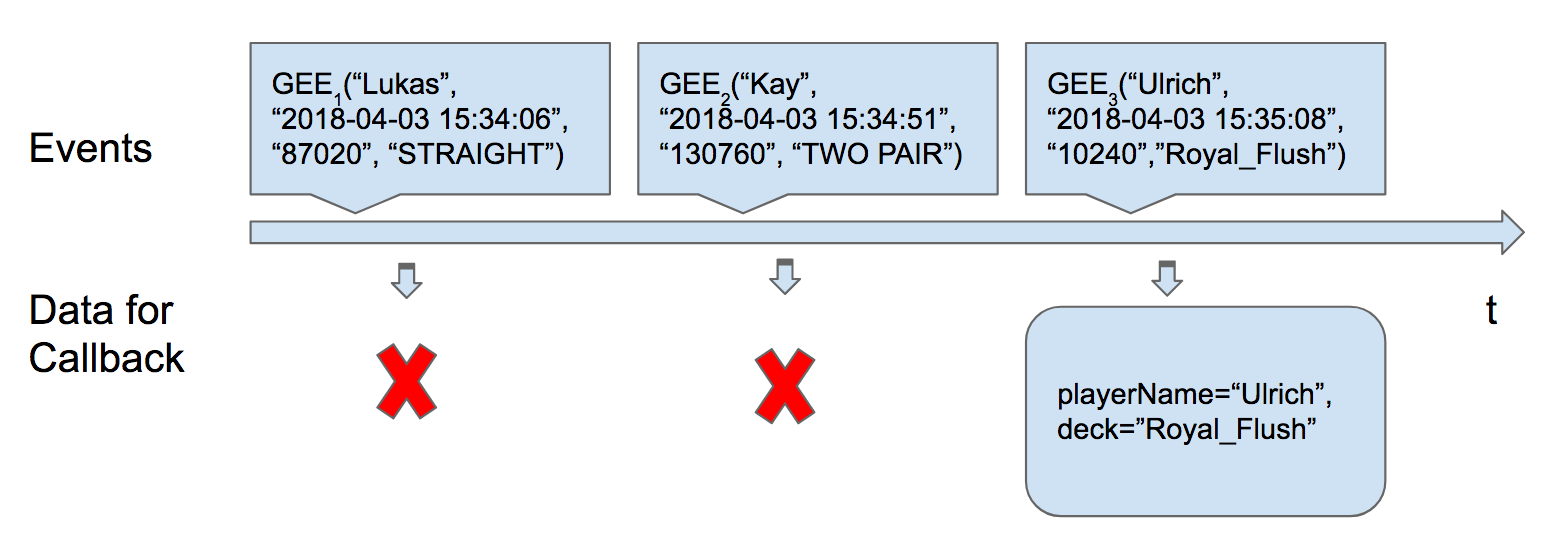
\includegraphics[width=\textwidth,height=\textheight, keepaspectratio]{images/statement_basic_filter.png}
	\caption{Ablauf gefilterte Selektion}
	\label{filter_select_img}
\end{figure}

\section{Aggregation}

Um zu erfahren, welcher Spieler wie oft gewonnen hat wird die Aggregationsfunktion \texttt{count(playerName)} verwendet.
\begin{lstlisting}[caption={Statement mit Aggregation}\label{aggregation_select},captionpos=b,language=SQL]

select playerName, count(playerName) as wins, deck from GameEndEvent

\end{lstlisting}
'' gespeichert.
Der Ablauf hierbei ist in Abbildung \ref{aggregation_select_img} veranschaulicht. 
Zudem sind weitere Aggregationsfunktionen wie \texttt{sum()} oder \texttt{avg()} in Esper verfügbar.
Im Casino fällt auf, dass sich die Spielenden der Vortage in den zu analysierenden Daten befinden. Um nur die Daten des aktuellen Tages auswerten zu können, sind Beschränkungen des auszuwertenden Ereignisstroms erforderlich. Die \acf{EPL} bietet hierfür sogenannte Data-Windows.
\cite{EsperRef2018}[9-10]

\begin{figure}[ht]
	\centering
	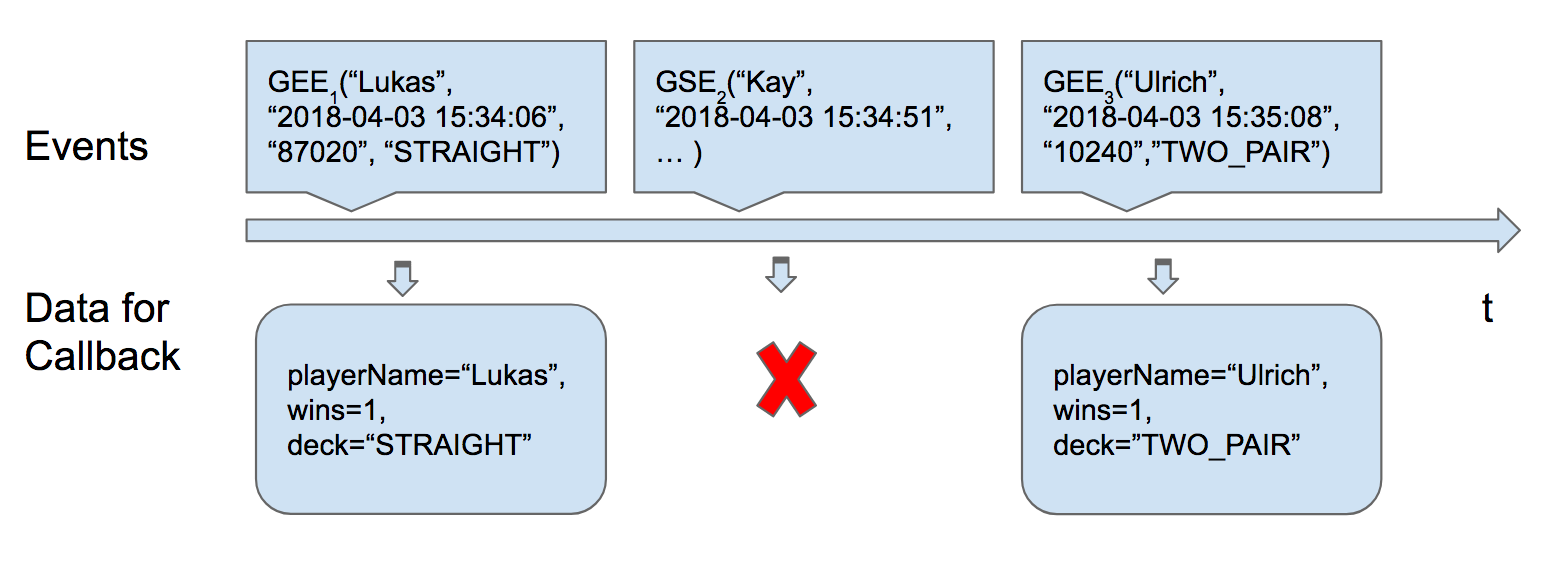
\includegraphics[width=\textwidth,height=\textheight, keepaspectratio]{images/statement_basic_aggregation.png}
	\caption{Ablauf Selektion mit Aggregation}
	\label{aggregation_select_img}
\end{figure}

\section{Data-Windows}
\label{Data-Windows}

\textbf{Data-Windows} werden in Esper verwendet, um Events im Bezug zueinander zu betrachten (Kausalität). Je nach Eigenschaft des \textbf{Data-Windows}, werden sie anhand von Kriterien (z.B. Anzahl oder Zeit) betrachtet.

Ein sehr einfaches \textbf{Data-Window} ist das nachfolgend dargestellte \textbf{Length Window}: 

\begin{figure}[ht]
	\centering
	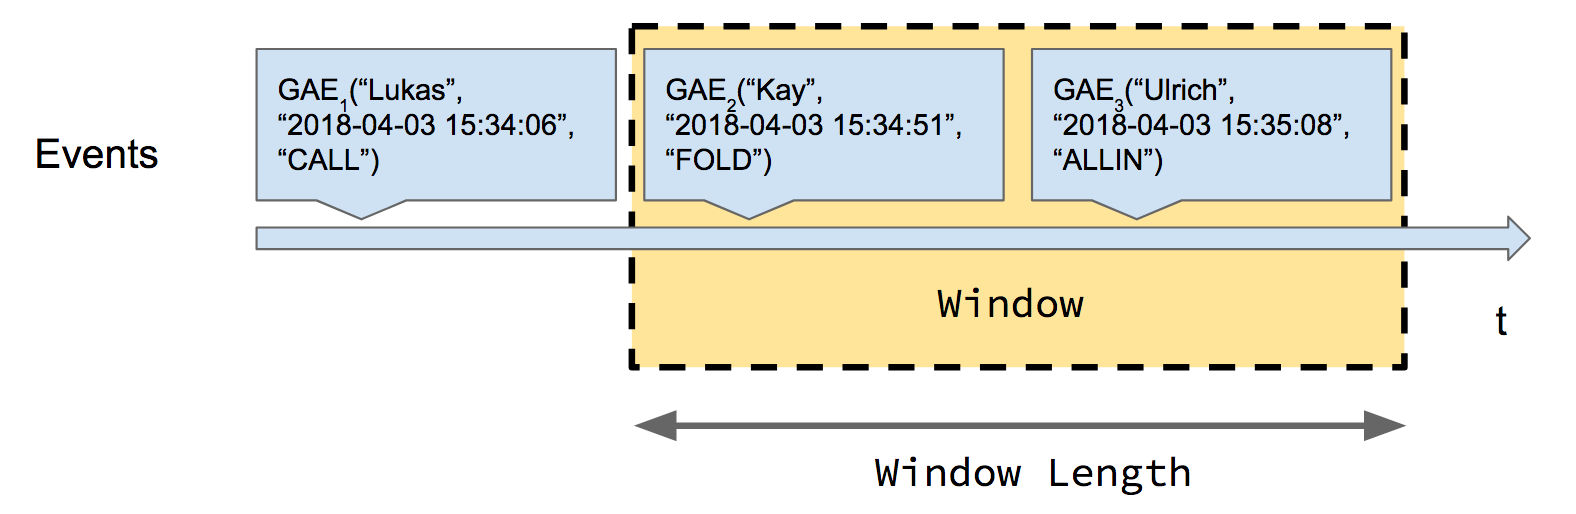
\includegraphics[width=\textwidth,height=\textheight,keepaspectratio]{images/data_window_length.png}
	\caption{Length Window}
	\label{LengthWindow}
\end{figure}

Dieses \textbf{Data-Window} wird mit einer Länge konfiguriert (in der Abbildung, ist der Wert 2), welche angibt, wie viele Events zusätzlich zum aktuellen betrachtet werden sollen. In diesem Fall würde das aktuelle und vorherige Event betrachtet werden.

Die Art des Events wird im Statement angegeben. Für das obige Beispiel könnte dies folgendermaßen aussehen:

\begin{lstlisting}[caption={Statement mit Length Window}\label{length_select},captionpos=b,language=SQL]

select * from GameActionEvent.win:length(2)

\end{lstlisting}

Wichtig ist an dieser Stelle anzumerken, dass das Statement des \textbf{Length Windows} erfüllt ist, sobald mindestens ein Event vom Typ \textbf{GameActionEvent} vorhanden ist. Dabei spielt die angegebene Länge keine Rolle. Nur wenn der Event-Strom mehrere passende Events beinhaltet, wird das \textbf{Length Window} ''gefüllt'' bis zu seiner maximalen Länge.

Ein \textbf{Data-Window} mit einem anderen Ansatz, ist das \textbf{Length-Batch Window}:

\begin{figure}[ht]
	\centering
	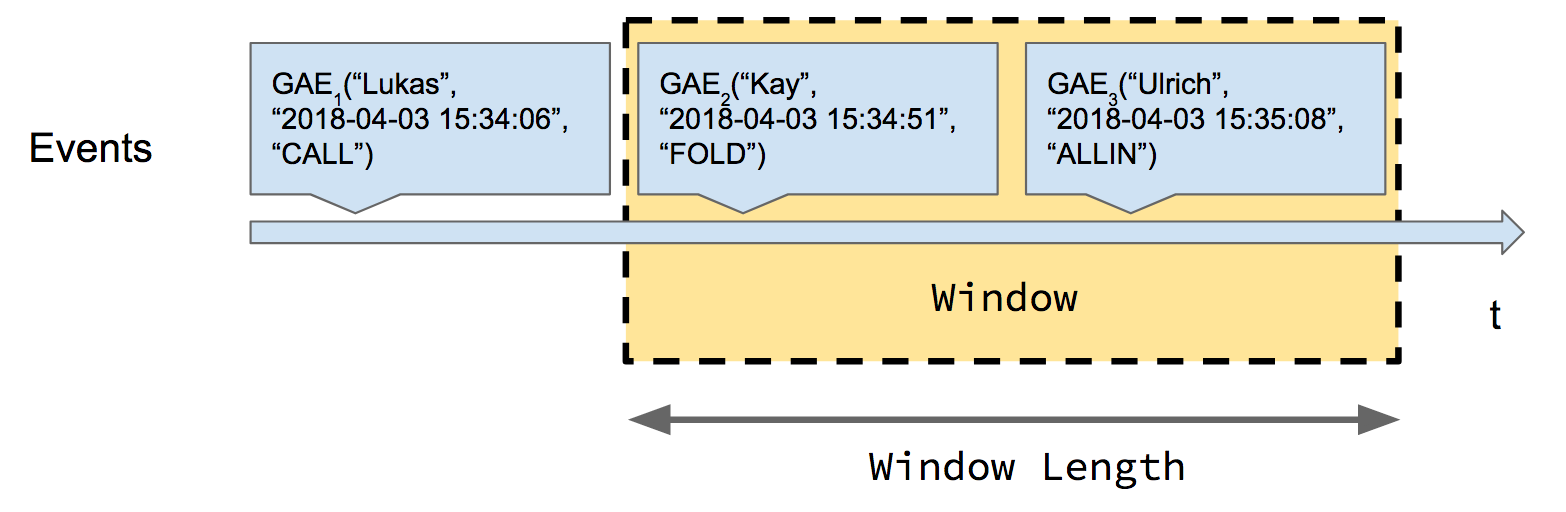
\includegraphics[width=\textwidth,height=\textheight,keepaspectratio]{images/data_window_length_batch.png}
	\caption{Length-Batch Window}
	\label{LengthBatchWindow}
\end{figure}

Dieses \textbf{Data-Window} verhält sich fast identisch zum \textbf{Length Window}, wird allerdings erst erfüllt, wenn genau so viele oder mehr Events im Event-Strom vorhanden sind, wie als Länge des \textbf{Data Windows} angegeben. Dadurch ist es möglich, Abfragen zu erstellen, die zuerst eine gewisse Anzahl an Events benötigen, um eine sinnvolle Weiterverarbeitung zu gewährleisten.

Neben dem betrachten der Anzahl von Events als Kriterium, gibt es auch die Möglichkeit der zeitlichen Betrachtung. Ein Beispiel hierfür ist das \textbf{Time Window}:

\begin{figure}[ht]
	\centering
	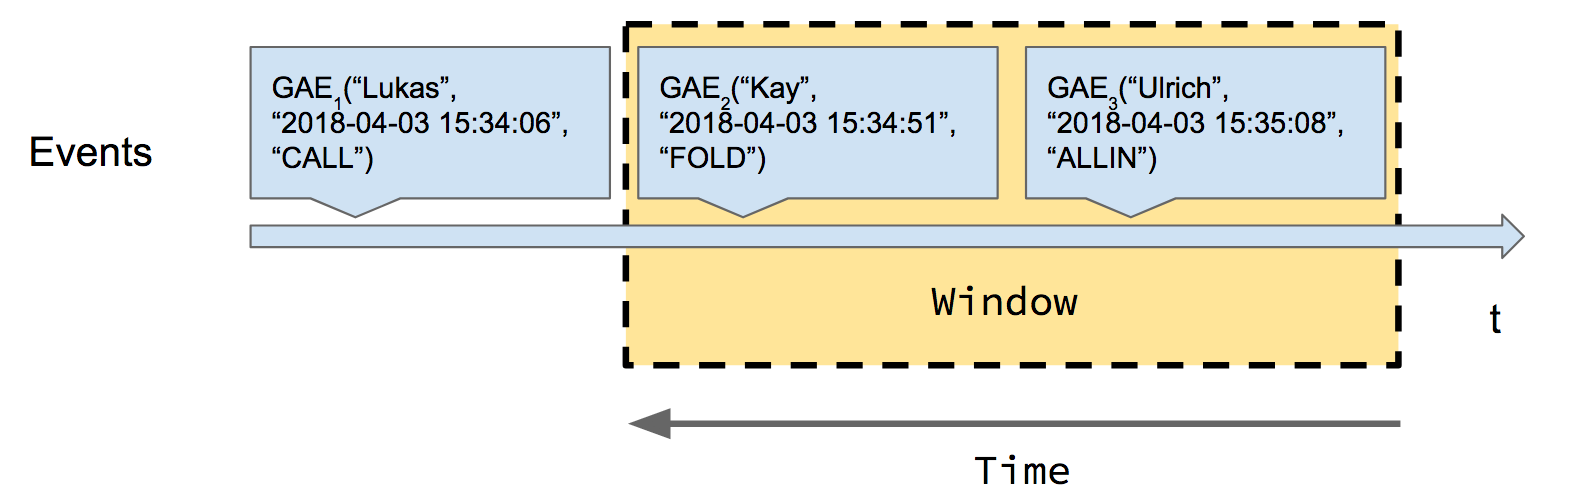
\includegraphics[width=\textwidth,height=\textheight,keepaspectratio]{images/data_window_time.png}
	\caption{Time Window}
	\label{TimeWindow}
\end{figure}

Bei diesem \textbf{Data-Window} werden alle Events innerhalb des konfigurierten Zeitabschnittes betrachtet.
Dabei wird stets vom aktuellen Zeitpunkt aus, anhand des angegeben Zeitwertes (z.B. 5 Sekunden), in die Vergangenheit gegangen. In anderen Worten, würden wir als Ergebnis das aktuelle Event erhalten und alle Events die bis zu 5 Sekunden vorher stattgefunden haben.

Zu Letzt gibt es auch ein \textbf{Data-Window} ohne Kriterium, das \textbf{Keep-All Window}:

\begin{figure}[ht]
	\centering
	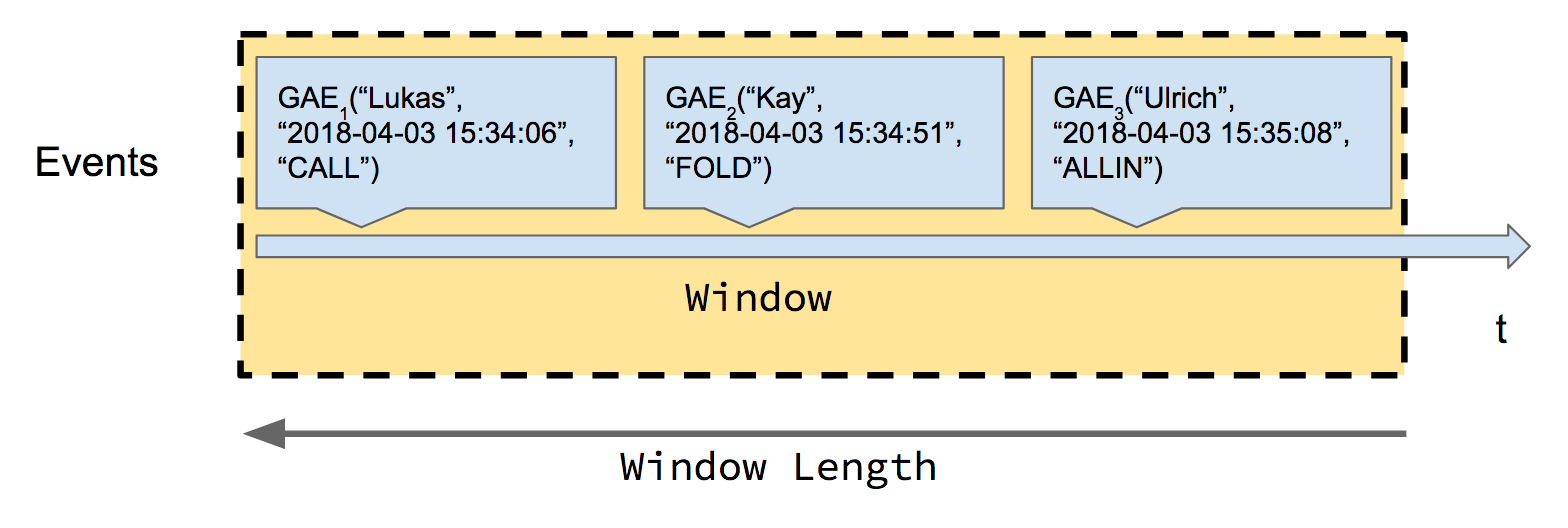
\includegraphics[width=\textwidth,height=\textheight,keepaspectratio]{images/data_window_keep_all.png}
	\caption{Keep-All Window}
	\label{KeepAllWindow}
\end{figure}

Dieses \textbf{Data-Window} ist erfüllt, sobald das erste Event im Event-Storm auftaucht. Es werden beliebig viele Events gesammelt und im Speicher gehalten.
Aufgrund von dem hohen Speicherverbrauch, sollte dieses nur eingesetzt werden, wenn eine kleine Event-Menge vorliegt und diese Gesamt Betracht werden sollen.

\section{Patterns}

Eine Alternative zu den Select-Satements stellen Abfragen nach Strukturen, sogenannte Patterns dar. Events, welche den Bedingungen entsprechen werden erfasst. Hierbei kommen verschiedene Elemente bei der Pattern-Definition zum Einsatz.
\cite{EsperRef2018}[25]

\begin{enumerate}
	\item \textbf{Kontrolloperator:} \texttt{every} definiert die Erstellung eines Pattern und regelt die Abarbeitung. Es wird alle(engl. every) auf das Ereignismuster zutreffende Ereignisse erfasst. Ein simples Pattern, welches alle Ereignisse vom Typ \texttt{GameActionEvent} erfasst, kann Quellcode \ref{basic_pattern} entnommen werden.
	Mit der \texttt{where}-Klausel können wie bei der Selektion weitere Bedingungen, definiert werden.
	
	\begin{lstlisting}[caption={Einfaches Pattern mit Where-Klausel}\label{basic_pattern}, captionpos=b,language=SQL]
	
	every GameActionEvent
	
	\end{lstlisting}
	
	\item \textbf{Logische Operatoren:} 
	Das Pattern kann, wie in Quellcode \ref{logic_pattern} veranschaulicht, durch logische Operatoren wie \texttt{and, or , not} zusammengesetzt werden. So kann wie in Quellcode \ref{logic_pattern} das Ereignismuster mit Bedingungen bestückt werden. In diesem Beispiel würden Events vom Typ \texttt{GameEnd} oder vom Typ \texttt{GameAction} erfasst werden.
	
	\begin{lstlisting}[caption={Pattern mit logischen Operatoren}\label{logic_pattern},captionpos=b,language=SQL]
	
	every a=GameActionEvent or b=GameActionEvent
	
	\end{lstlisting}
	
	\item \textbf{Nachfolge-Operator:}
	Der Nachfolge-Operator \texttt{->} tritt ein wenn das davor, gefolgt vom danach definierten Ereignis eintrifft. In Quellcode \ref{follow_pattern}  werden alle Endevents betrachtet, welche auf ein Aktionsevent folgen. Die Bedingung trifft zu, wenn der vorangegangene Zug ein Spielausstieg(\texttt{action = "FOLD"}) war.
	Wie im Quellcode zu erkennen ist, werden die Ereignisse in Variablen \texttt{a, b} gespeichert(bspw. \texttt{a=GameAction}). So können die Werte im nächsten Schritt weiterverwendet werden. Im Beispiel wird das Folgeevent (\texttt{b=GameEnd(a.playerName != b.playerName)}) überprüfen ob der Spieler-Name ungleich dem vorherigen ist und im Erfolgsfall erfasst. Auf diese Art lassen sich komplexe bedingte Ereignismuster definieren.
	
	\begin{lstlisting}[caption={Pattern mit Follow-Operator }\label{follow_pattern},captionpos=b,language=SQL]
	
	every a = GameActionEvent(action="FOLD") -> b =
	 GameEndEvent(a.playerName != b.playerName)
	
	\end{lstlisting}
	
	\item \textbf{Bedingungen:}
	Um Grenzen zu definieren, nach welcher das Pattern geprüft wird, dient die \texttt{where}-Klausel. Nach ihr können verschiedene Bedingungen, durch Konstellationen der Operatoren, angegeben werden.
	Meisten werden Vergleichsoperatoren wie \texttt{=, < , > , >=, <=, !=, <>, is null, is not null} und logische Kombinationen wie\texttt{and, or} verwendet. So können Ereignisse in Korrelation gestellt und ausgewertet werden. Die \texttt{where}- Klausel kann auch bei der Selektion verwendet werden.
	
	\item \textbf{Überwacher} (engl. Observer):
	Um Ereignisströme zu überwachen werden Observer verwendet, welche beispielsweise in einem Zeitintervall oder zu einem Zeitpunkt agieren. Sie können nach der \texttt{where}-Klausel angegeben werden. Beispielsweise kann ein Timer mit Intervall, durch \texttt{timer:interval} definiert werden. Ein Zeitpunkt wird
	mit \texttt{timer:at} festgelegt, eine Zeitspanne mit \texttt{timer:within}. Für das Casino wird der Überwacher auf ein Zeitintervall eines Werktages gesetzt, um nur die Ereignisse des aktuellen Tages zu erhalten. So fließen die historischen Daten nicht verfälschend in die Auswertung mit ein.
	
	\begin{lstlisting}[caption={Pattern mit Observer }\label{observer_pattern},captionpos=b,language=SQL]
	
	every a = GameActionEvent(action="FOLD") -> b =
	GameEndEvent(a.playerName != b.playerName)
	where timer:within(28800 seconds)
	
	\end{lstlisting}
	
\end{enumerate}


\section{Partitions}

Esper bietet die Möglichkeit Abfragen zu partitionieren.
Hierzu wird ein zeitlicher Context mit \texttt{create context} erstellt.
\texttt{start} definiert den Start-, \texttt{end} den Endzeitpunkt.
Mit \texttt{after 28800 sec} wir die Dauer dynamisch auf eine Zeitspanne von acht Stunden gesetzt. Verwendet wird der erzeugte Context mit texttt{context OneWorkDay}. Diese Deklaration sorgt dafür, dass sich das darauffolgende \texttt{select}-Statement auf die Partition bezieht.
In Quellcode \ref{partitioned_pattern} wird mit dem ersten Statement eine achtstündige Partition erstellt. Diese wird in der zweiten Zeile verwendet, um die Spieler- und Spielzugnamen aller Aktionen eines Arbeitstagen zu erfassen.
\cite{EsperRef2018}[18]

\begin{lstlisting}[caption={Partitioniertes Pattern}\label{partitioned_pattern},captionpos=b,language=SQL]

create context OneWorkDay start @now end after 28800 sec

context OneWorkDay select playerName, action from GameActionEvent

\end{lstlisting}

\section{Kombinierte Statements}

